%%%%%% 第一题
% \chapter{第一题}

%%%%%%题目描述


%%%%%%解题思路
\chapter{给定电荷密度的分布函数,求解泊松方程,得到电势分布.}

\section{题目描述}

已知三维空间中轴对称的电荷分布函数为
\begin{equation}
f(r,\theta)=\frac { 0.8 } { 1 + e ^ { ( r - r 0 ) / 0.6 } } \left[ \mathrm { c } \cdot \mathrm { fm } ^ { - 3 } \right]
\end{equation}

\begin{align}
&r _ 0 = 10.0 \left( 1 + 1.0 Y _ { 2 } ^0+ 0.5 Y _ { 3 }^0 \right) \mathrm { fm }\\
&{ Y _ { 2 } ^ { 0 } ( \theta , u ) = \frac { 1 } { 4 } \sqrt { \frac { 5 } { \pi } } \left( 3 \cos ^ { 2 } \theta - 1 \right) } \\ 
&{ Y _ { 3 } ^ { 0 } ( \theta , u ) = \frac { 1 } { 4 } \sqrt { \frac { 7 } { \pi } } \cdot \left( 5 \cos ^ { 3 } \theta - 3 \cos \theta \right) }
\end{align}

\section{题目分析}

球坐标系中的泊松方程展开式为:

\begin{align}
\nabla ^ { 2 } u = \frac { 1 } { r ^ { 2 } } \frac { \partial } { \partial r } \left( r ^ { 2 } \frac { \partial u } { \partial r } \right) + \frac { 1 } { r ^ { 2 } \sin \theta } \frac { \partial } { \partial \theta } \left( \sin \theta \frac { \partial u } { \partial \theta } \right) + \frac { 1 } { r ^ { 2 } \sin ^ { 2 } \theta } \frac { \partial ^ { 2 } u } { \partial  \phi ^ { 2 } } = -f ( \rho , \theta , \phi )
\end{align}

由于电荷分布函数呈轴对称, 因此对应的解应该也与$\phi$无关. 因此问题降维至二维情形,我们只需要考虑对$r$与$\theta$划分格点.泊松方程可以简化为:

\begin{align}
\nabla ^ { 2 } u = \frac { 1 } { r ^ { 2 } } \frac { \partial } { \partial r } \left( r ^ { 2 } \frac { \partial u } { \partial r } \right) + \frac { 1 } { r ^ { 2 } \sin \theta } \frac { \partial } { \partial \theta } \left( \sin \theta \frac { \partial u } { \partial \theta } \right)= -f ( r , \theta )
\end{align}

\section{求解方法}

我们解决 PDE 的大致思路是:利用差分方法对偏微分方程进行展开表示,配合格点法,将偏微分方程变化为 $N*M$ 个线性方程组, 线性方程组的解$u_{i,j}\,i = 1,2,\ldots, N, j=1,2,\ldots, M$为原偏微分方程的每一点上的数值解. 为解一个线性方程组,我们常用的方式是 Jacobi 迭代, 或 Gauss-Seidel 迭代法.

\subsection{格点法}

将$r$与$\theta$分别划分为$N+1$和$M+1$个格点.令$r$的取值范围为$1\sim R\cdot N/(N+1)$,$\theta$的取值范围为$\pi/(M+1)\sim \pi\cdot M/(M+1)$.格点的大小分别为$\Delta r=\frac {R} {M+1}$及$\Delta \theta=\frac {\pi} {N+1}$. 径向$r$和角向$\theta$分别可以离散化为:

\begin{align}
&r_i=i\Delta r\quad\quad i=1,2,\cdots,N,N+1\\
&\theta_j=j\Delta \theta\quad\quad j=1,2,\cdots,M,M+1\\
&u(r_i,\theta_j)=u_{i,j}\\
&f(r_i,\theta_j)=f_{i,j}
\end{align}

\subsection{有限差分法}

有限差分法建立在格点法离散后的格点基础之上,它利用格点周围的若干个格点对一阶偏微分和二阶偏微分进行表示.一阶偏导数和二阶偏导数的表示分别为:
\begin{align}
& \frac { \partial u } { \partial r } = \frac { u _ { i + 1,j } - u _ { i -1 , j} } {2\Delta r}\\
& \frac { \partial u } { \partial \theta }  = \frac { u _ { i, j + 1 } - u _ {i,  j -1} } {2\Delta \theta}\\
& \frac { \partial ^ { 2 } u } { \partial r ^ { 2 } }  =  \frac { u _ { i + 1, j } - 2 u _ { i, j } + u _ { i - 1, j} }  { (\Delta r)^2}\\
&\frac { \partial ^ { 2 } u } { \partial \theta ^ { 2 } } =  \frac { u _ {i, j + 1 } - 2 u _ {i, j } + u _ {i, j - 1} }  { (\Delta \theta)^2}
\end{align}

因此,将偏微分导数换成这些格点差分表示,泊松方程可写成如下形式:
\begin{align}
 {\frac { u _ { i + 1 , j } - 2 u _ { i j } + u _ { i - 1 , j } } { ( \Delta r ) ^ { 2 } } + \frac { u _ { i + 1 , j } - u _ { i - 1 , j } } { \Delta r } +  \frac { u _ { i , j + 1 } - 2 u _ { i j } + u _ { i , j - 1 } } {r^2 ( \Delta \theta ) ^ { 2 } } + \cot \theta \frac { u _ { i , j + 1 } - u _ { i , j - 1 } } { 2r^2 \Delta \theta } = - f _ { i , j } }
\end{align}

而又有$r=i\Delta r$,$\theta=j\Delta \theta$:
\begin{equation}
\begin{split}
{i^2( u _ { i + 1 , j } - 2 u _ { i j } + u _ { i - 1 , j } )+ i (u _ { i + 1 , j } - u _ { i - 1 , j } ) &+ \frac{1}{(\Delta \theta)^2} ( u _ { i , j + 1 } - 2 u _ { i j } + u _ { i , j - 1 } )\\ 
&+ \frac{\cot(j\Delta\theta)}{2\Delta\theta}( u _ { i , j + 1 } - u _ { i , j - 1 } )  = -i^2(\Delta r)^2 f _ { i , j } }
\end{split}
\end{equation}

合并同类项并整理,得到:

\begin{equation}
\begin{split}
{(1+\frac{1}{i^2})u _ { i + 1 , j }&+ (1-\frac{1}{i^2})u _ { i - 1 , j }+(-2-\frac 2i^2{(\Delta \theta)^2}) u _ { i , j } \\ 
&+ (\frac{1}{i^2(\Delta \theta)^2}+\frac{\cot(j\Delta\theta)}{2i^2\Delta\theta})  u _ { i , j + 1 }+ (\frac{1}{i^2(\Delta \theta)^2}-\frac{\cot(j\Delta\theta)}{2i^2\Delta\theta}) u _ { i , j - 1 } = -(\Delta r)^2 f _ { i , j } }
\end{split}
\end{equation}


\subsection{矩阵表示与边界条件}

这是一个未知量有$N\times M$个的线性方程组,系数矩阵$\textbf A$的阶数为:$(NM)\times(NM)$.我们将未知量排成一列,并将同一个$\theta$(同一个$j$)上的$N$个未知量简记为$u_j$,有:

$$
v=
\begin{bmatrix}
u_1\\
\vdots\\
u_j\\
\vdots\\
u_M
\end{bmatrix}
,\quad
u_j=
\begin{bmatrix}
u_{1,j}\\
\vdots\\
u_{i,j}\\
\vdots\\
u_{M,j}
\end{bmatrix}
$$

我们利用矩阵来表示这个线性方程组,系数矩阵为$A$,是一个$MN\times MN$的方阵, $v$和$b$分别是求解的向量和非齐次项,他们都是长度为$NM$的列向量:
\begin{equation}
Av = b
\end{equation}

等式右边的非齐次项$b$可以表示为
$$
b=
\begin{bmatrix}
b_1\\
\vdots\\
b_j\\
\vdots\\
b_M
\end{bmatrix}
,\quad
b_j=
\begin{bmatrix}
-(\Delta r)^2 f _ { 1 , j } }\\
\vdots\\
-(\Delta r)^2 f _ { i , j } }\\
\vdots\\
-(\Delta r)^2 f _ { N , j } }\\
\end{bmatrix}
$$

这里其实蕴含了我们所取的边界条件.首先考虑$r$的边界条件.在$r\rightarrow 0$时,$i=1$,可以得到:

\begin{equation}
\begin{split}
{2u _ { 2 , j }+(-2-\frac 2{(\Delta \theta)^2}) u _ {1, j }+ (\frac{1}{(\Delta \theta)^2}+\frac{\cot\theta}{2\Delta\theta})  u _ { 1 , j + 1 }+ (\frac{1}{(\Delta \theta)^2}-\frac{\cot(j\Delta\theta)}{2\Delta\theta}) u _ { 1 , j - 1 } = -(\Delta r)^2 f _ { 1, j } }
\end{split}
\end{equation}

可以发现由于$u_{0,j}$前面的系数计算得为0,从而方程中不存在这一项.因此我们不需要$i=0$处的边界条件.

在$r$很大的时候,我们取$u_{N,j}=0$,即$r\rightarrow\inf$时电势等于0.由此可以得到$i=N$处的方程为:
\begin{equation}
\begin{split}
N(N-1)u _ { N - 1 , j }+(-2N^2-\frac 2{(\Delta \theta)^2}) u _ { N , j } 
+ (\frac{1}{(\Delta \theta)^2}+\frac{\cot(j\Delta\theta)}{2\Delta\theta})  u _ { N , j + 1 }\\+ (\frac{1}{(\Delta \theta)^2}-\frac{\cot(j\Delta\theta)}{2\Delta\theta}) u _ { N , j - 1 } = -i^2(\Delta r)^2 f _ { N , j } 
\end{split}
\end{equation}

系数矩阵$A$可以表示为:
$$
A=
\begin{bmatrix}
T-D-W_1&D+W_1\\
D-W_2&T-2D&D+W_2\\
&\ddots&\ddots&\ddots\\
&&D-W_j&T-2D&D+W_j\\
&&&\ddots&\ddots&\ddots\\
&&&&D-W_{M-1}&T-2D&D+W_{M-1}\\
&&&&&D-W_M&T-D+W_M\\
\end{bmatrix}
$$

矩阵$A$的构建也利用到了我们的边界条件,我们规定了$\theta$的边界条件为Neumann边界条件: $( \frac { \partial u } { \partial \theta } )_0=0$,$( \frac { \partial u } { \partial \theta } )_\pi=0$  换言之,按照有限差分法,应该是: $u_{i,0}=u_{i,1}$, 和$u_{i,M}=u_{i,M+1}$,这蕴含着电势在两个边界都是分别连续的.因此,当$j=1$时的有限差分方程为:
\begin{equation}
\begin{split}
{i(i+1)u _ { i + 1 , 1 }+ i(i-1)u _ { i - 1 , 1 }+(-2i^2-\frac 1{(\Delta \theta)^2}-\frac{\cot(\Delta\theta)}{2\Delta\theta}) u _ { i , 1 }\\+ (\frac{1}{(\Delta \theta)^2}+\frac{\cot(\Delta\theta)}{2\Delta\theta})  u _ { i , 2 }+= -i^2(\Delta r)^2 f _ { i , 1 } }
\end{split}
\end{equation}

当$j=M$时, 接近于$\pi$的边界为:
\begin{equation}
\begin{split}
{i(i+1)u _ { i + 1 , N }+ i(i-1)u _ { i - 1 , N }+(-2i^2-\frac 1{(\Delta \theta)^2}+\frac{\cot(N\Delta\theta)}{2\Delta\theta}) u _ { i , N }\\+
(\frac{1}{(\Delta \theta)^2}-\frac{\cot(N\Delta\theta)}{2\Delta\theta}) u _ { i , N - 1 } = -i^2(\Delta r)^2 f _ { i , j } }
\end{split}
\end{equation}

故矩阵$A$的第一行分块矩阵为$T-D-W_1$和$D+W_1$, 而最后一行分块矩阵为$T-D-W_M$和$D-W_M$.

分块矩阵$T$、$W$、$D$的大小均为$N\times N$, 而有$M$个这些矩阵, 所以$A$的总大小也是$NM\times NM$.$\;\;T$为一个三对角矩阵,$W$和$D$均为对角矩阵,具体形式为:

$$
T=
\begin{bmatrix}
-2&1+\lambda_1\\
1-\lambda_2&-2&1+\lambda_2\\
&\ddots&\ddots&\ddots\\
&&1-\lambda_i&-2&1+\lambda_i\\
&&&\ddots&\ddots&\ddots\\
&&&&1-\lambda_{N-1}&-2&1+\lambda_{N-1}\\
&&&&&1-\lambda_N&-2\\
\end{bmatrix}
$$

其中: $\lambda_i = 1/i, i = 1,2,\ldots, N$.

$$
W_j=\mathrm{diag}\left(\frac{\cot(j\theta)}{2i^2\cdot\Delta\theta}}\right)=
\begin{bmatrix}
\frac{\cot(j\theta)}{2\Delta\theta}}\\
&\frac{\cot(j\theta)}{8\Delta\theta}}\\
&&\ddots\\
&&&\frac{\cot(j\theta)}{2(N-1)^2\Delta\theta}}\\
&&&&\frac{\cot(j\theta)}{2N^2\Delta\theta}
\end{bmatrix}
$$
$$
D=\mathrm{diag}\left(\frac1{ i^2 (\Delta \theta)^2}\right)=
\begin{bmatrix}
\frac1{(\Delta \theta)^2}\\
&\frac1{4(\Delta \theta)^2}\\
&&\ddots\\
&&&\frac1{(N-1)^2(\Delta \theta)^2}\\
&&&&\frac1{N^2(\Delta \theta)^2}
\end{bmatrix}
$$

\subsection{Gauss-Seidel 迭代方法}

我们解线性方程组的一般方法是: 利用Gauss-Seidel 迭代方法对系数矩阵$A$进行迭代计算. 对于一个含有$n$个未知量及$n$个等式的如下线性方程组:

\begin{equation}
\begin{split} 
a _ { 11 } \cdot x _ { 1 } + a _ { 12 } \cdot x _ { 2 } + \ldots + a _ { 1 n } \cdot x _ { n } & = b _ { 1 } \\
 a _ { 21 } \cdot x _ { 1 } + a _ { 22 } \cdot x _ { 2 } + \ldots + a _ { 2 n } \cdot x _ { n } & = b _ { 2 } \\ 
 \vdots & = \\ a _ { n 1 } \cdot x _ { 1 } + a _ { n 2 } \cdot x _ { 2 } + \ldots + a _ { n n } \cdot x _ { n } & = b _ { n }
 \end{split} 
\end{equation}

为了求这个方程组的解 ${\displaystyle {\vec {x}}}$ ,我们使用迭代法. $k$用来计量迭代步数.给定该方程组解的一个近似值$ {\displaystyle {\vec {x}}^{\,k}\in \mathbb {R} ^{n}} $.在求k+1步近似值时,我们利用第$m$个方程求解第$m$个未知量.在求解过程中,所有已解出的$k+1$步元素都被直接使用,这一点与雅可比法不同.对于每个元素可以使用如下公式:

\begin{equation}
x _ { m } ^ { k + 1 } = \frac { 1 } { a _ { m m } } \left( b _ { m } - \sum _ { j = 1 } ^ { m - 1 } a _ { m j } \cdot x _ { j } ^ { k + 1 } - \sum _ { j = m + 1 } ^ { n } a _ { m j } \cdot x _ { j } ^ { k } \right) , \quad 1 \leq m \leq n
\end{equation}

重复上述的求解过程,可以得到一个线性方程组解的近似值数列: ${\displaystyle {\vec {x}}^{0},{\vec {x}}^{1},{\vec {x}}^{2},\ldots } $.在该方法收敛的前提下,此数列收敛于 $ \vec{x}$.

为了保证该方法可以进行,主对角线元素 $ {\displaystyle a_{mm}}$需非零. 可知我们的系数矩阵$A$符合以上条件,因此可以利用该迭代方法来进行求解.

\section{结果分析}

我们选择线度$R = 20$, 格点数$N=100, M=70$.那么格点数为$N\times M=7000$, 系数矩阵$A$的阶数为$7000\times 7000$. 设置最大迭代次数为15000次,当精度达到$TOL=1\times 10^{-2}$时,提前退出迭代.

运行算法,得到在第7747次迭代后,精度达到0.00998,各点电势按照前面所述的顺序按照一列排列,记录在solution.txt 当中.我们利用 matlab 进行绘图,得到结果如下:
\begin{figure}[htp]
    \centering
    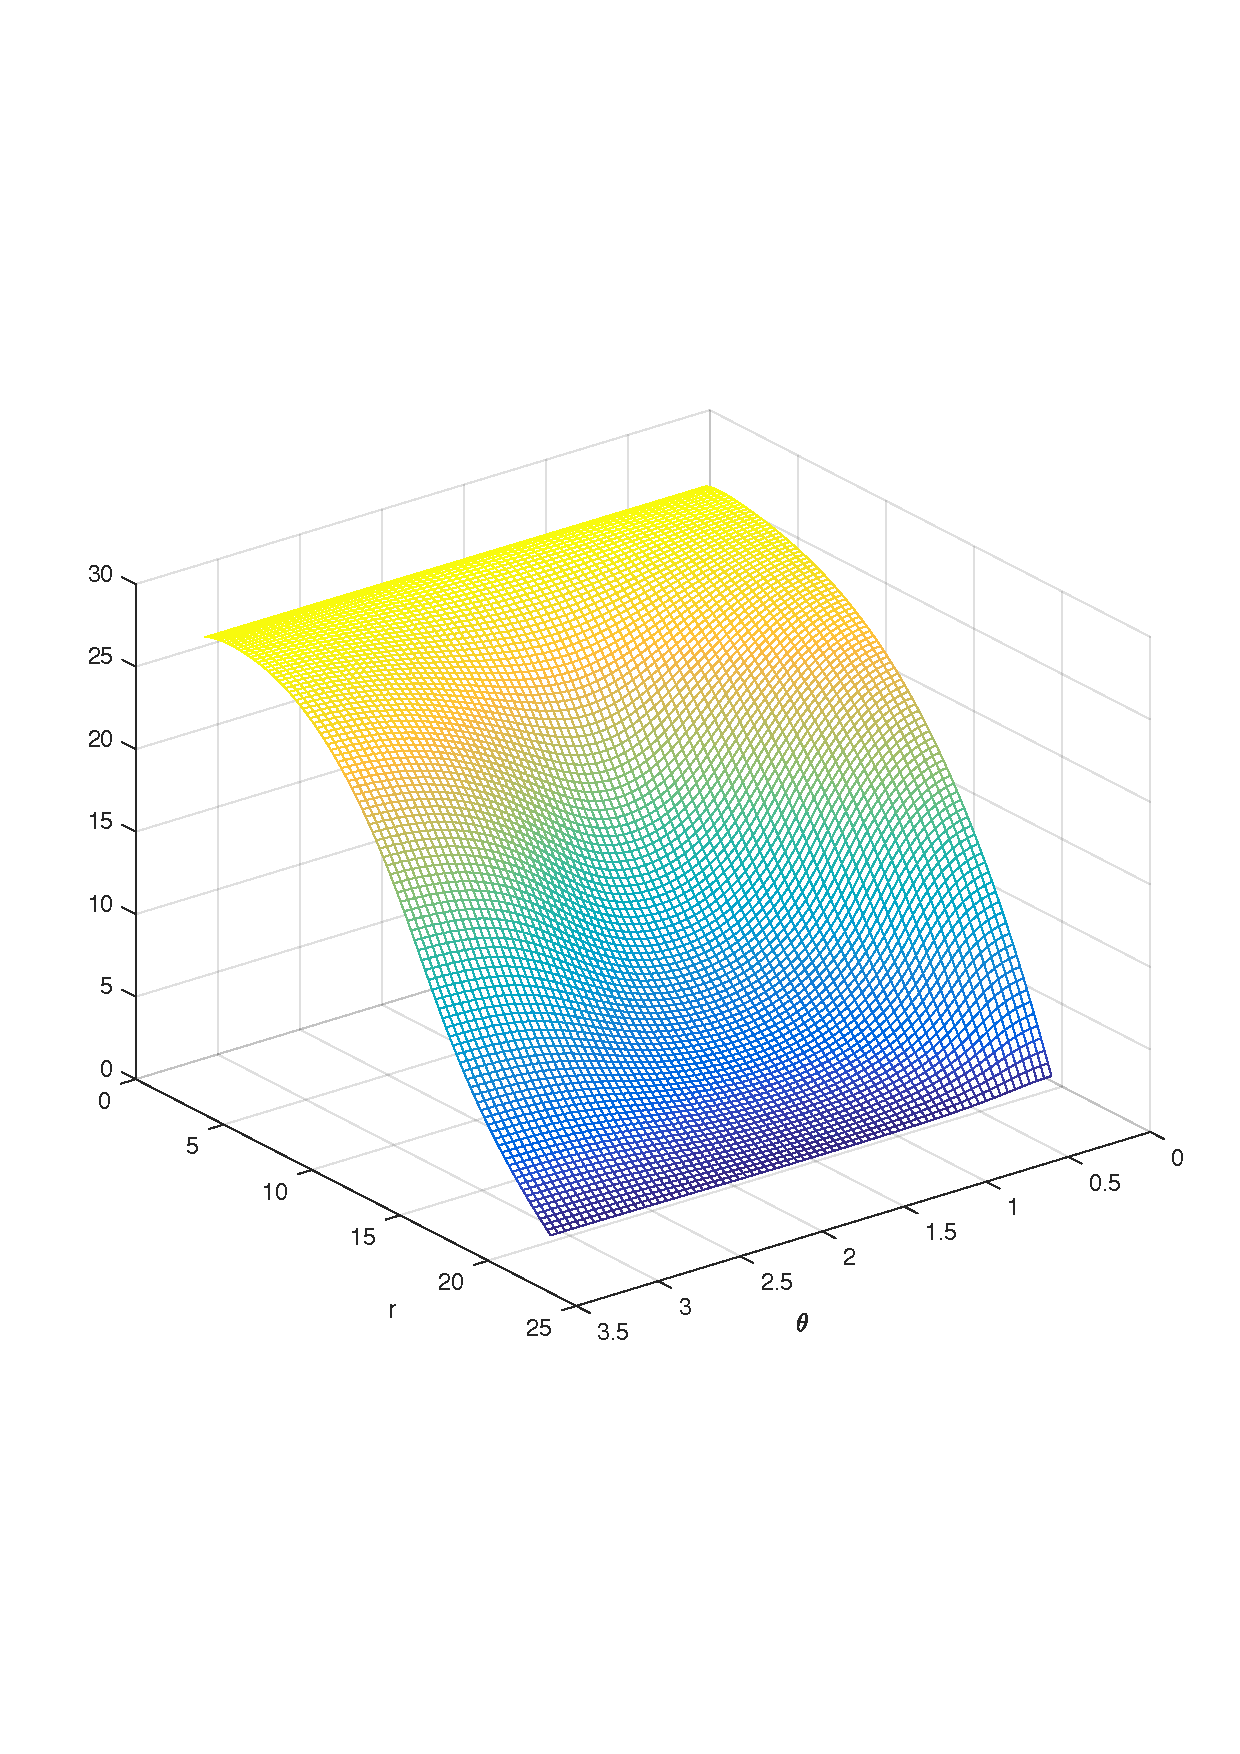
\includegraphics[scale = 0.5]{pic/1.pdf}
    \caption{$r-\theta$电势分布图1}
\end{figure}

\begin{figure}[htp]
    \centering
    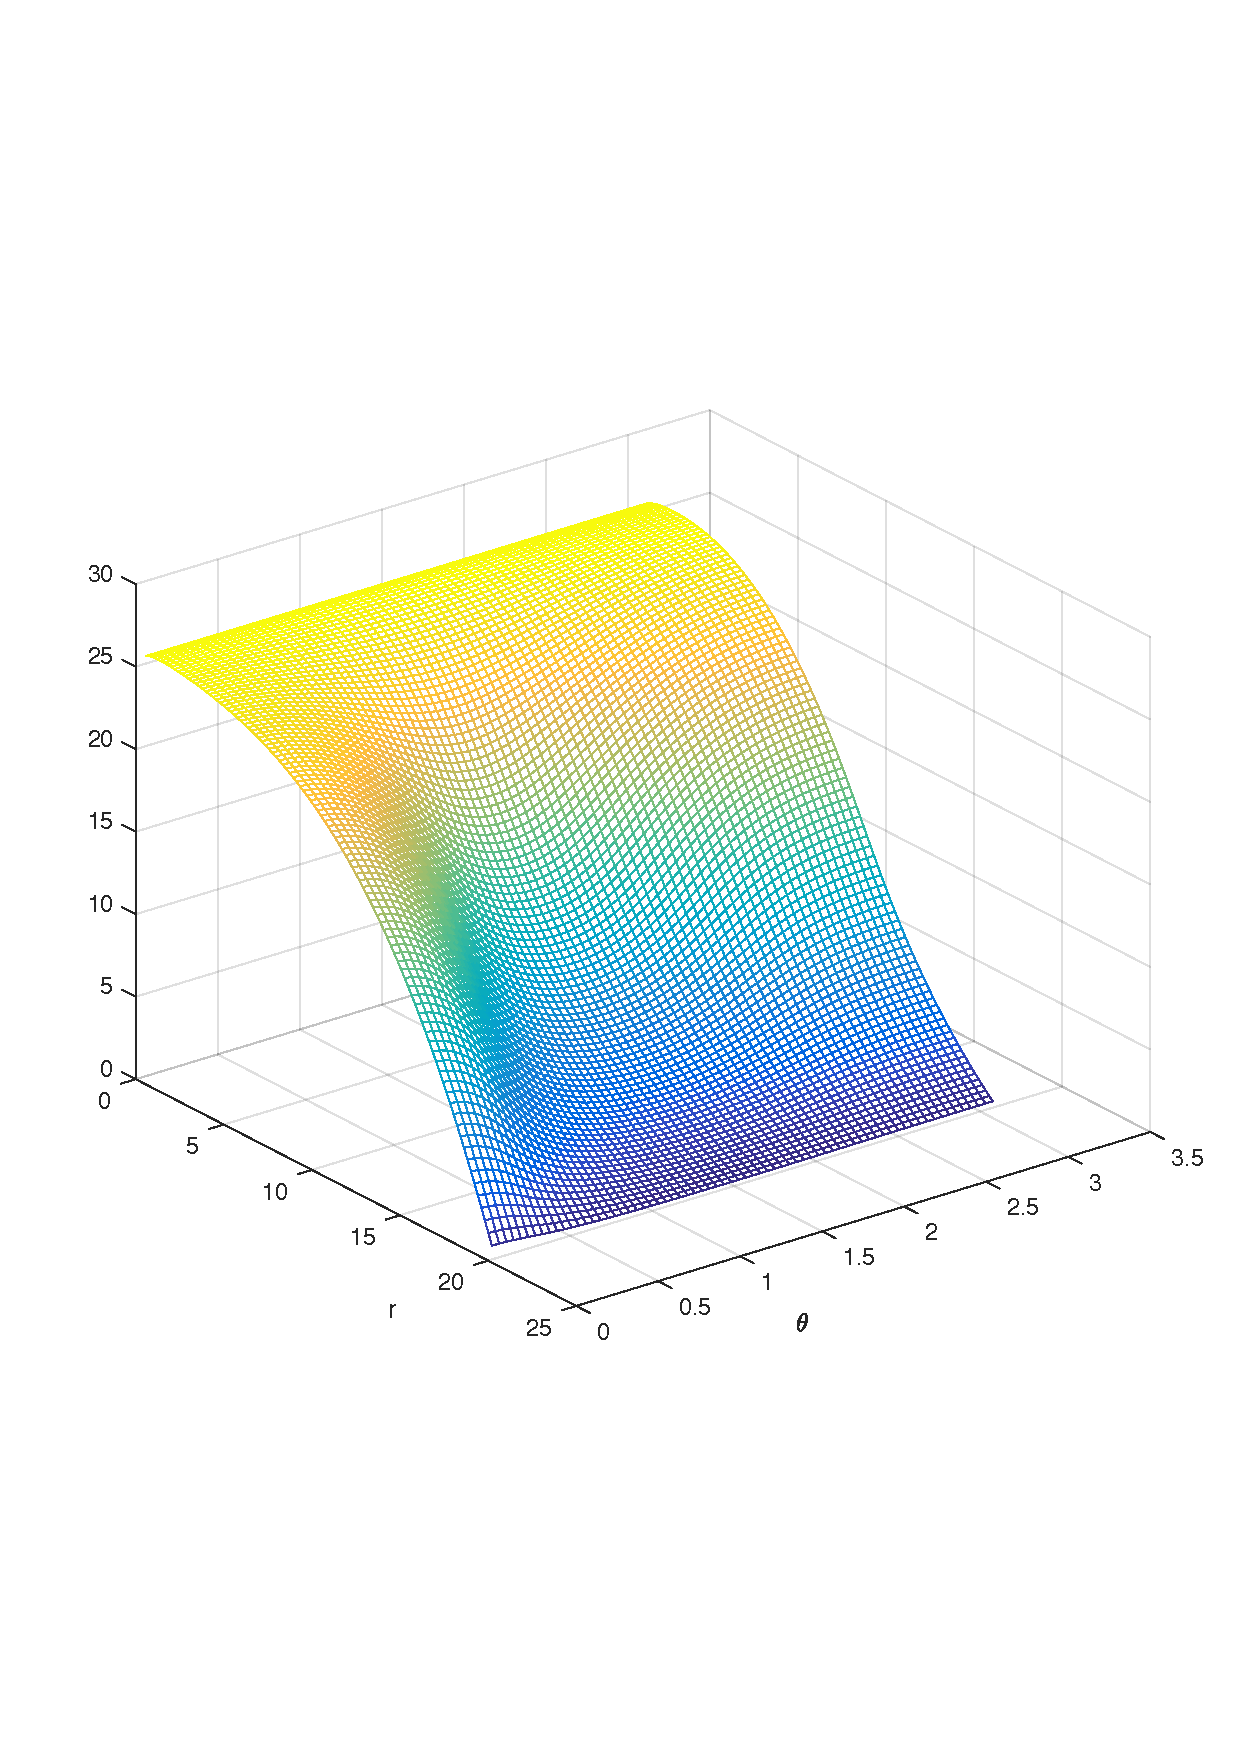
\includegraphics[scale =0.50]{pic/2.pdf}
    \caption{$r-\theta$电势分布图2}
\end{figure}

可以看到我们的电势分布呈瀑布状,而中间有一个明显的“凹陷”部分.经两幅图对比可知,凹陷处比较靠近$\theta$较小的部分.而电势变化的总体趋势是随着$r$的增加逐渐减小, 随$\theta$增大的过程中,电势先减小后增大.
